\label{app4}





\section{Simplified inverse kinematics}

The controller demands that the configuration of the actuator is known at each sampling instant. Therefore the modal coordinates need to be calculated based on the sensor data. Since the configuration of the actuator is approximated with a single shape function. The inverse kinematic problem can implicitly be solved with the constant curvature approach. The sensor output, which is the x,y position in the plane, and the orientation of the tip of the actuator $\theta$ can be used to determine modal coordinates $\epsilon$ and $\kappa$. At each sampling instant this inverse kinematics are determined. Based on the modal coordinates the Jacobian matrix can be updated, which in its turn is used in determining the new control input. The simplified kinematics are shown in Figure \ref{fig:simpkin}.

\begin{figure}[H]
    \centering
    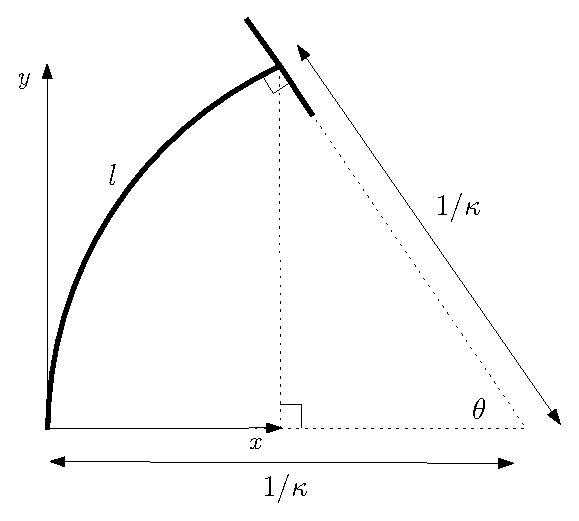
\includegraphics[width = 0.5\textwidth]{Figures/Chapter5/fbdkinematics.eps}
    \caption{Schematic drawing of the actuator to determine mapping from configuration space to task space}
    \label{fig:simpkin}
\end{figure}

From above figure the following forward kinematic relations follow as,


\begin{equation}
    y = \frac{1}{\kappa}\sin(\theta) \hspace{15pt} \text{and} \hspace{15pt}    x = \frac{1}{\kappa}[1-\cos(\theta)] \hspace{15pt} \text{with} \hspace{10pt}   \theta = l \kappa.
\end{equation}

where $l$ is the length of the backbone curve of the manipulator given by $l = (1+\epsilon)L$. Accordingly, the modal coordinates can then be calculated by,

\begin{equation}
    \kappa = \frac{\sin(\theta)}{y} \hspace{15pt} 	\land \hspace{15pt}  \kappa = \frac{1 -\cos(\theta)}{x} \hspace{15pt} \text{and} \hspace{10pt} \epsilon = \frac{\theta}{\kappa L} -1,
\end{equation}

where it should be noted that for small angles it is more accurate to use $\kappa$ based on the $\sin(\theta)$.



\label{app:chap5}

\section{Position acquisition from pixel to world coordinates}

\begin{figure}[H]
    \centering
    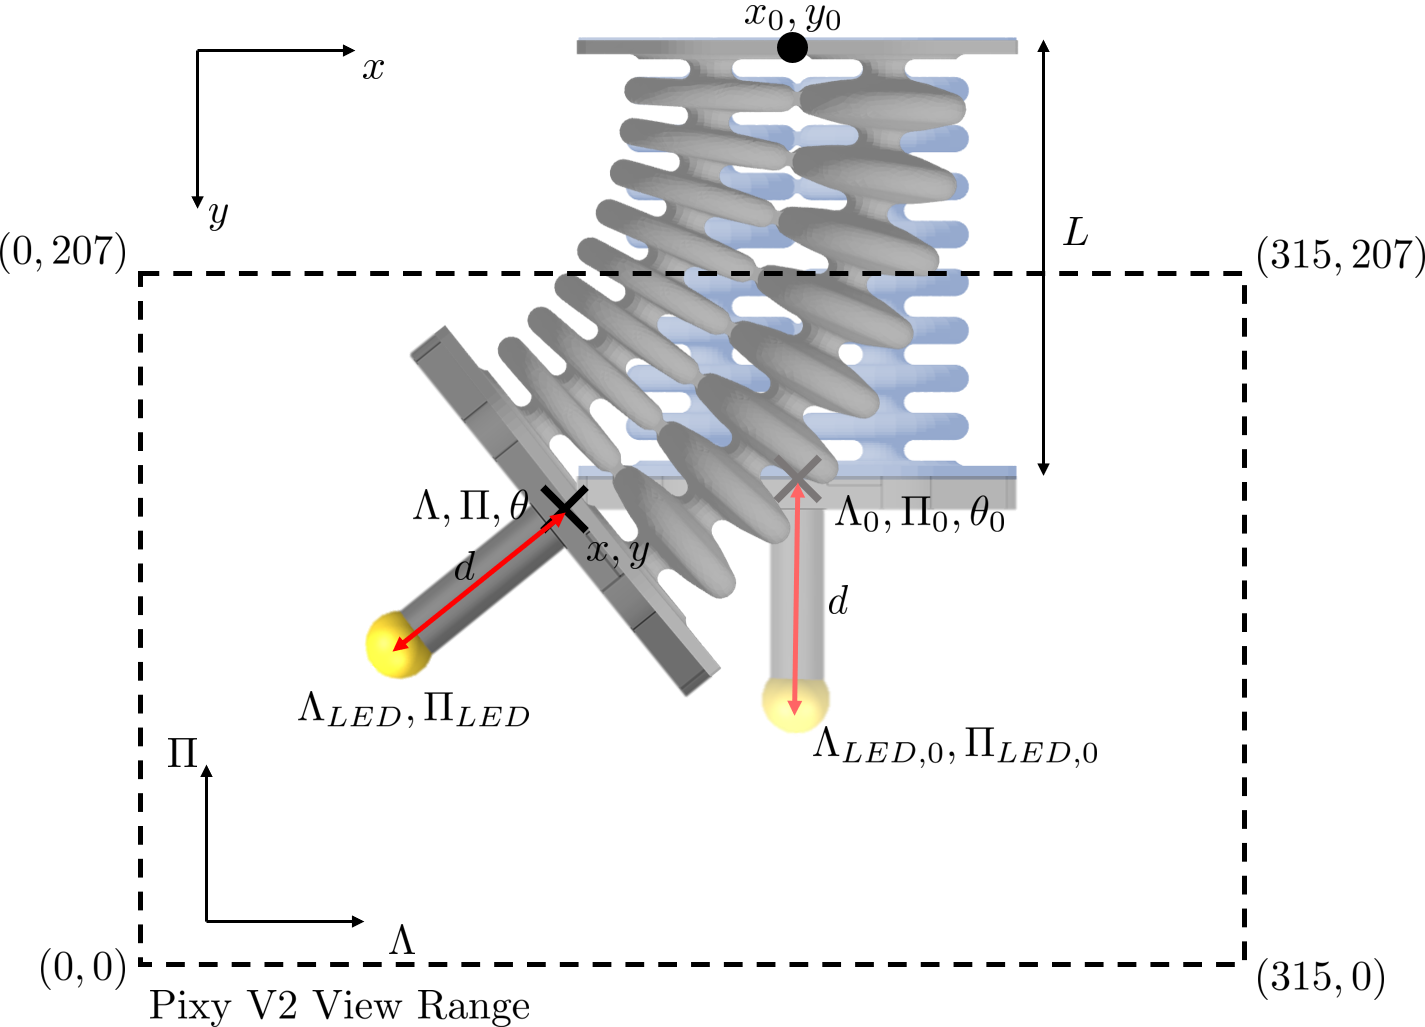
\includegraphics[width = 0.95\textwidth]{Figures/Appendix5/pix2w.png}
    \caption{Vision system coordinate frame.}
    \label{figapp5:px2w}
\end{figure}


Figure \ref{figapp5:px2w} displays the vision system coordinate frame, where the dotted lines mark the pixel window. The resolution of the vision system is 207$\times$315, as indicated by the corner coordinates. The pixel values of the end-effector are denoted by $(\Lambda,\Pi)$. The position of the $LED$ marker in pixel coordinates are given by $(\Lambda_{LED},\Pi_{LED})$. Consider the origin of the soft robot in world frame coordinates given by $(x_0,y_0)$. Note that this position can be outside of the vision system's viewing range. The initial end-effector position in pixel coordinates is given by,


\begin{equation}
    \Lambda_0 = \Lambda_{LED,0} + \frac{d}{px2w} \sin(\theta_0) \hspace{20pt} \text{and} \hspace{20pt} \Pi_0 = \Pi_{LED,0} + \frac{d}{px2w} \cos(\theta_0),
\end{equation}

where $d$ is the offset between the LED marker and the end-effector, $px2w$ a constant mapping pixel coordinates to world coordinates. The initial angle is given by $\theta_0$. Likewise, the actual position of the end-effector during operation is given by,


\begin{equation}
    \Lambda = \Lambda_{LED} + \frac{d}{px2w} \sin(\theta) \hspace{20pt} \text{and}  \hspace{20pt}  \Pi = \Pi_{LED} + \frac{d}{px2w} \cos(\theta).
\end{equation}

Based on the difference between actual and initial position in pixel coordinates, the position in world coordinates can be obtained by, 

\begin{equation}
    x = (\Lambda-\Lambda_0)px2w \hspace{20pt} \text{and} \hspace{20pt} y = L - (\Pi - \Pi_0)px2w. 
\end{equation}




